\chapter{Fundamentação Teórica}

% fundamentação teórica
%---------------------------------------------------------------------------------------------------------------------
\section{Redes Sociais}

Redes sociais online têm atraído milhões de usuários que integraram essas plataformas nos seus dia-a-dia. Essas plataformas são bastante variadas nos seus propósitos e culturas, enquanto algumas são direcionadas a um publico diversificado, outros são focados em atrair pessoas que compartilham características comuns. De acordo com \cite{boyd_social_2007} um site de rede social é um serviço online que permite que seus usuários:

\begin{enumerate}
    
    \item \textbf{Construam um perfil público ou semi-publico dentro do sistema}: Este perfil é gerado utilizando uma série de formulários que podem conter algumas questões pessoais sobre o participante como idade, nome, localidade, interesses ou profissão. Alguns sites permitem que usuários personalizem seus perfis permitindo a adição de mídias como fotos e vídeos, ou modifiquem a interface da página de perfil;
    
    \item \textbf{Articulem uma lista de outros usuários que compartilham uma conexão}: Após se juntar a uma rede social, os usuários podem identificar outras pessoas no sistema, que eles possuam uma conexão. Esse relacionamento pode variar em nomenclatura dependendo do site, os termos "Amigos" e "Contatos" estão entre os mais comuns. O relacionamento pode ser de duas maneiras: \textbf{(1) bidirecional}, onde a conexão só é formada com a confirmação de "amizade" entre os dois usuários da rede, ou \textbf{(2) unidirecional}, indicando que uma pessoa pode possuir a outra na lista de contato, mas a recíproca pode não ser verdadeira, como o recurso de ``seguir'' utilizado pela plataforma \emph{Twitter};
    
    \item \textbf{Organizem e cruzem sua lista de contatos com as listas feitas por outros usuários}: Isso pode ser alcançado de várias maneiras, entre elas: (1) a lista de contatos do usuário possui um link direcionando para a lista de contatos de cada usuário em sua rede, permitindo a visualização e a interação com diferentes redes sociais, (2) o próprio site propõe usuários com interesses semelhantes, através de um algoritmo que cruza informações obtidas através de seus perfis. Geralmente são utilizadas uma dessas estratégias, as duas, ou mistura delas.
    
\end{enumerate}

\cite{boyd_social_2007} apontam que os sites de redes sociais geralmente fornecem um mecanismo para que os usuários deixem mensagens uns para os outros de forma pública ou privada. Além disso, alguns sites fornecem varias outras funcionalidades como: compartilhamento de fotos, vídeos, mensagens, artigos, \emph{urls}, escrita de blog, etc. Variando de acordo com o objetivo principal de cada site.

Segundo \cite{haythornthwaite_social_2005} o que faz esses sites tão interessantes para o público é sua capacidade de permitir que os usuários interajam com as redes sociais uns dos outros. Isso pode resultar em conexões entre pessoas, que não aconteceriam de outra maneira. Porém este não é o objetivo, e essas conexões frequentemente acontecem entre pessoas que possuem um "laço latente", uma conexão offline. \cite{boyd_social_2007} discutem que em muitas das grandes redes sociais os participantes não necessariamente procuram novas conexões, o principal objetivo deles é se comunicar com pessoas que já fazem parte de sua rede social. Porém, para enfatizar a característica de organização e articulação destes serviços, eles são chamados de "Sites de Redes Sociais".


%---------------------------------------------------------------------------------------------------------------------
\section{Fake News}

\cite{robert_darnton_true_2017} mostra que o termo \emph{Fake News}(FN) não é novo, e aponta que fenômenos de desinformação em massa existem a séculos e com muitos exemplos no decorrer história da humanidade. As definições encontradas na literatura são variadas, o dicionário de Cambridge\footnote{https://dictionary.cambridge.org/dictionary/english/fake-news. Acessado em 24 de Janeiro, 2018} define \emph{Fake News} como: 

\begin{quote}
    "False stories that appear to be news, spread on the internet or using other media, usually created to influence political views or as a joke"
    \footnote{Tradução do autor: "Histórias falsas que parecem ser notícias, disseminadas pela Internet ou em outro smeios de comunicação, normalmente criadas para influenciar visões políticas ou com caráter humorístico"}
\end{quote}

Já \cite{allcott_social_2017} afirmam que FN são:
\begin{quote}
    "News articles that are intentionally and verifiably false, and could mislead readers"
    \footnote{Tradução do autor: "Notícias intencionalmente falsas, podem ser verificadas como falsas, porém tem poder de enganar as pessoas que estão lendo"}
\end{quote}

A definição de \cite{allcott_social_2017} exclui alguns termos que tem sido relacionados a Fake News: (1) erros cometidos por acidente; (2) rumores que não se originaram de um artigo em particular; (3) teorias da conspiração (essas são por natureza difíceis de verificar como verdadeiras ou falsas); (4) Sátiras que dificilmente seriam confundidas como verdade; (5) falsas declarações de políticos; (6) relatórios que são tendenciosos mas não completamente falsos. Entretanto \cite{tandoc_defining_2017} discutem um termo mais abrangente e propõem um \emph{framework} baseado em definições do termo utilizadas em artigos científicos publicados entre 2003 e 2017, que é utilizado para construir uma tipologia de FN. Para entender como funciona o \emph{framework} precisamos apresentar primeiramente as seis maneiras de operacionalização de \emph{fake news} encontradas pela pesquisa de \cite{tandoc_defining_2017}:

\begin{enumerate}
    \item \textbf{Sátiras de notícias:} Utiliza-se de humor ou exagero para apresentar o conteúdo á audiência. Entretanto, o humor utilizado nessas notícias é apenas um artifício para entreter o público, e não visa descaracterização na veracidade da informação apresentada;
    
    \item \textbf{Paródias de notícias:} Muito semelhante as sátiras, as paródias também utilizam-se de humor para transmitir conteúdo. Porém, nas paródias é normal que a informação seja retorcida e que dados inventados sejam inseridos pelo bem do humor; 
    
    \item \textbf{Fabricação de notícias:} São artigos sem embasamento em fatos que se mascaram como notícias reais, tentam transmitir legitimidade e buscam ludibriar o público. A diferença entre a fabricação e a paródia de notícias está no entendimento existente entre o público e o autor.  Na paródia, o público sabe que está lendo uma notícia falsa e de caráter humorístico, na fabricação o autor busca confundir o leitor, que fica com dificuldade para decernir a veracidade do conteúdo apresentado.
    
    \item \textbf{Manipulação de multimídia:} Enquanto as outras categorias se referem a conteúdos textuais, nessa é descrita a manipulação gráfica de imagens e vídeos;
    
    \item \textbf{Publicidade e relações públicas:} Nesta categoria materiais publicitários sob a aparência de notícias genuínas. Isso acontece quando profissionais de relações públicas adotam práticas e/ou aparência de jornalistas para inserir mensagens persuasivas nos meios de comunicação. As famosas manchetes \emph{clickbait}\footnote{"Articles, photographs, etc. on the internet that are intended to attract attention and encourage people to click on links to particular websites". https://dictionary.cambridge.org/us/dictionary/english/clickbait. Acessado em 24 de Janeiro, 2018}\footnote{Tradução do autor:"Artigos, fotos, etc. na Internet que possuem a intenção de atrair atenção e encorajar as pessoas a clicar em um link em websites particulares} que utilizam o formato de noticias convencionais, mas direcionam o público para um conteúdo comercial são exemplos de FN dessa categoria;
    
    \item \textbf{Notícias tendenciosas ou propagandas políticas:} Notícias que são criadas por entidades políticas para influenciar a opinião pública. O propósito dessas notícias é beneficiar uma organização, figura pública ou governo. Similares aos anúncios publicitários, porém as propagandas geralmente são uma mistura de fatos com uma narrativa tendenciosa. São alguns exemplos de propaganda: Matérias tendenciosas e artigos com conteúdo persuasivo e unilateral.
\end{enumerate}

Analisando as categorias apresentadas nota-se que todas tentam parecer notícias legitimas, se apossando de formatos e visuais consagrados por mídias convencionais e se aproveitando da credibilidade que essas possuem. Para mapear os tipos de \emph{Fake News} \cite{tandoc_defining_2017} ainda propõe a utilização de dois domínios: \textbf{(1) facticidade}, se referindo ao grau em que a notícia se baseia em fatos reais, e \textbf{(2) intenção imediata do autor}, uma referência ao propósito do autor com a notícia, se o autor planeja enganar o público com a sua notícia ou não.

A figura \ref{fig:topologia_fn} mostra a formação de um plano cartesiano utilizando os dois domínios mencionados, este plano pode ser utilizado para mapear as diferentes categorias de FN.

\begin{figure}[!htb]
\centering
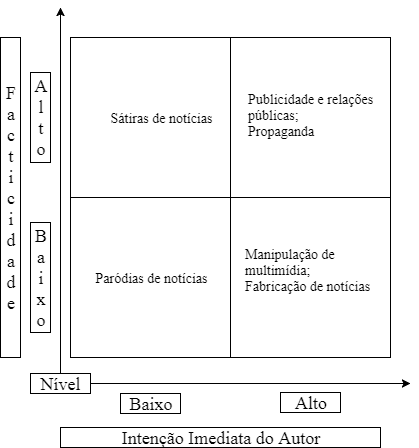
\includegraphics[width=10cm]{2-fundamentacao/typology_fake_news.png}
\caption{Tipologia de \emph{Fake News}.}
\label{fig:topologia_fn}
\end{figure}

Conclui-se então que apesar de ser muito utilizado na mídia (\cite{liliana_bounegru_field}, o termo"\emph{Fake News}" é muito abrangente e possui diferentes definições dependendo do estudo e do contexto, mas é possível mapear essas definições que podem ser utilizadas como base no nosso trabalho.

%---------------------------------------------------------------------------------------------------------------------
\section{Autoridade Cognitiva}

Em seu livro, \emph{Second-hand Knowledge: An Inquiry into Cognitive Authority} \cite{Wilson1983} apresenta a teoria da Autoridade Cognitiva (AC), desenvolvida através de um estudo da natureza social humana. Em seu trabalho ele afirma que o ser humano constrói conhecimento de duas maneiras: 
\begin{enumerate}
    \item \textbf{Primeira mão}: onde a pessoa constrói conhecimento através das suas próprias experiências;
    \item \textbf{Segunda mão}: onde a pessoa constrói conhecimento através das experiências de outras pessoas. Sendo que ele fundamenta sua teoria da Autoridade Cognitiva nesta maneira de adquirir conhecimento. 
\end{enumerate}

Wilson acredita que tudo que as pessoas conhecem do mundo fora do curto alcance das suas vidas, é o que outras pessoas contam. Ele afirma que tudo é boato, mas que nem todos os boatos são iguais, existem alguns confiáveis, aqueles que "sabem o que estão falando", e apenas esses contam como autoridades cognitivas. Ele usa o termo autoridade cognitiva para descrever alguém que influencia, que as pessoas consideram apropriado. É diferente de uma autoridade administrativa provinda de uma posição hierárquica imposta ou concedida. Portanto uma AC é alguém cujas capacidades e competências foram reconhecidas por outro indivíduo.

Wilson discute que existem vários elementos que são levados em consideração quando definimos Autoridades Cognitivas:

\begin{enumerate}
    \item \textbf{Envolve um relacionamento entre no mínimo dois atores}: uma pessoa precisa ser reconhecida por outra para ser uma autoridade cognitiva, ou reconhecer outra para que esta seja uma AC;
    
    \item \textbf{Existe um nível de AC}: uma pessoa pode ter um nível alto ou baixo de autoridade;
    
    \item \textbf{É relativo à uma área de interesse}: uma pessoa pode ter um nível alto de AC em determinado assunto, mas não ter em outro que escapa da sua linha de conhecimento;
    
    \item \textbf{AC é relacionada à credibilidade}: pois só concedemos autoridade à quem julgamos dignos de confiança, uma fonte de informação que não é considerada digna será então naturalmente descartada.
\end{enumerate}

Se uma pessoa utilizar como base de conhecimento apenas aquilo que ela vivencia, essa pessoa passa a ter ideias muito limitada, pois esse individuo tem uma período de vida curto onde não é possível experimentar tudo. É utilizando os conhecimentos de segunda mão aprendidos através da experiência de outros que uma pessoa pode expandir sua visão de mundo. Entretanto, é importante destacar que Wilson não diz que conhecimento de segunda-mão é mais importante do que vivenciar experiências diretamente (primeira mão), mas apoia que é melhor confiar em alguém do que ter uma visão limitada sobre um assunto fora de sua área de interesse.
